\section{Nutzen des Algorithmus an Beispielen} % (fold)
\label{sec:PermutationExamples}
Aus der Vorlesung von Herrn Stroetmann und dem begleitenden Skript \autocite{github-stroetmann:online} ist bekannt, dass sich Puzzle aus Abb.\ref{fig:Ex1_start} lösen, also in den Zielzustand aus Abb.\ref{fig:Ex1_end} überführen lässt.\\
\begin{minipage}{\linewidth}
	\begin{minipage}[t]{0.45\linewidth}
		\begin{figure}[H]
			\centering
			\includegraphics[width=\linewidth,keepaspectratio]{img/Ex1_start.png}
			\captionsetup{format=plain, indention=0pt}
			\caption{Beispiel1: Startzustand eines 4x4-Puzzles nach figure 2.20 aus \autocite{github-stroetmann:online} \label{fig:Ex1_start}}
		\end{figure}
	\end{minipage}
	\hfill
	\begin{minipage}[t]{0.45\linewidth}
		\begin{figure}[H]
			\centering
			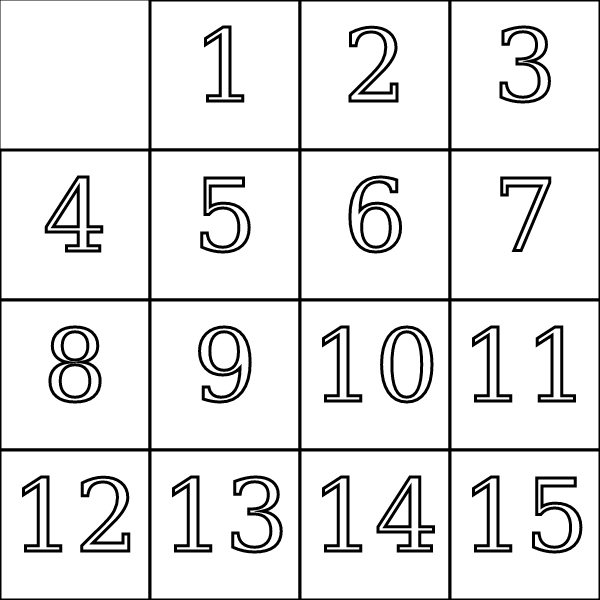
\includegraphics[width=\linewidth,keepaspectratio]{img/End_Puzzle_Stroetmann.png}
			\captionsetup{format=plain, indention=0pt}
			\caption{\label{fig:Ex1_end}Beispiel1: Zu erreichender Zielzustand für das Puzzle nach figure 2.20 aus \autocite{github-stroetmann:online}}
		\end{figure}
	\end{minipage}
\end{minipage}\WNL%
Der Algorithmus aus dem vorherigen Abschnitt schätzt diese Puzzles ebenfalls als Lösbar ein.\\
\begin{figure}[H]
	\begin{enumerate}
		\item[S1.1] Konvertierung der Puzzle-Zustände in Zahlenreihen
		\begin{align*}
		start_{ex1} = \{0,1,2,3,4,5,6,8,14,7,11,10,9,15,12,13\} \\
		end_{ex1} = \{0,1,2,3,4,5,6,7,8,9,10,11,12,13,14,15\}
		\end{align*}
		\item[S1.2] Notwendige Transpositionen $T_{ex1}$ um $start_{ex1} zu sortieren:$
		\begin{align*}		
		T_{ex1} = \{(8,7),(14,8),(14,9),(11,10),(14,12),(15,13)\}\\
		%0,1,2,3,4,5,6,8,14,7,11,10,9,15,12,13 (8,7)
		%0,1,2,3,4,5,6,7,14,8,11,10,9,15,12,13 (14,8)
		%0,1,2,3,4,5,6,7,8,14,11,10,9,15,12,13 (14,9)
		%0,1,2,3,4,5,6,7,8,9,11,10,14,15,12,13 (11,10)
		%0,1,2,3,4,5,6,7,8,9,10,11,14,15,12,13 (14,12)
		%0,1,2,3,4,5,6,7,8,9,10,11,12,15,14,13 (15,13)
		%0,1,2,3,4,5,6,7,8,9,10,11,12,13,14,15
		\left\vert T_{ex1}\right\vert = 6 \rightarrow \texttt{Parität} = 0	
		\end{align*}
		\item[S1.3] Anzahl der Notwendigen Züge $z_{ex1}$ um das Leerfeld von der Postion aus dem Startzustand(Koordinaten $(0,0)$ ) an die Postion des Zielzustandes (Koordinaten $(0,0)$) zu verschieben.
		\begin{align*}		
		z_{ex1} = \left | 0 - 0 \right | + \left | 0 - 0 \right |\\
		z_{ex1} = 0 \rightarrow \texttt{Parität} = 0
		\end{align*}	
		\item[S1.4] Die Paritäten stimmen überein, das Puzzle ist Lösbar.	
	\end{enumerate}
	\caption{Beispiel1: Anwendung des Algorithmus \label{fig:Ex1_algo}}
\end{figure}
Dazu wird wie in Abb.\ref{fig:Ex1_algo} schrittweise vorgegangen. Zunächst werden, wie im Abschnitt \ref{sec:PuzzleToList} und in Schritt 1 (S1.1) dargestellt, die Zustände in Zahlenreihen konvertiert.
Anschließend werden die Paritäten ermittelt (S1.2 und S1.3). Zunächst die Parität der Anzahl notwendiger Transpositionen und anschlie"send die Parität benötigter Züge um die Leerstelle korrekt zu platzieren. Im abschlie"senden Schritt (S1.4) werden die ermittelten Paritäten verglichen. In diesem Beispiel stimmen diese Paritäten über ein. Das Beispiel ist also lösbar.\WNL%


%Loyd
%Endzustände

